% Chapter X

\chapter{Error Correction} % Chapter title

\label{ch:name} % For referencing the chapter elsewhere, use \autoref{ch:name} 

The next part of the simulation will be the error correction scheme. In order to keep the program initially as simple as possible a variant of Jaewoo Joo's measurement based error correction scheme  using two auxilary qubits to create a 'triangle state' instead of the 'pentagon state's used in Joo's paper \citep{joo_error-correcting_2009}. This error correction scheme is convenient as it can be extended to larger size logical qubits easily so the correlation between fault tolerance and qubit number can be examined.

%----------------------------------------------------------------------------------------

\section{Logical qubits}

The first step towards simulation of the error correction scheme for measurement based quantum computation requires the definition of a logical state which represents a quantum state for which the information is distributed amongst multiple qubits. Following the work in 'Error - correcting one - way quantum computation with global entangling gates' \citep{joo_error-correcting_2009} we establish a logical state based on three qubits, rather than the five in the paper, to form a triangle state through three CZ operations. In doing so we obtain the unitary operator that will allow for conversion of three qubits in the  + state to the logical + state.

\begin{multline}
\hat{U} (t) =
exp\Bigg(-i \phi \bigg( 
\frac{1 - \sigma^{1}_{z}}{2} \frac{1 - \sigma^{2}_{z}}{2}\mathbb{1} \\
+ \frac{1 - \sigma^{1}_{z}}{2} \mathbb{1} \frac{1 - \sigma^{3}_{z}}{2}
+ \mathbb{1}\frac{1 - \sigma^{2}_{z}}{2} \frac{1 - \sigma^{3}_{z}}{2}
\bigg)\Bigg) \\
\end{multline}

Expanding out this expression gives:

\begin{multline}
\hat{U} (t) = exp(-\frac{i \phi}{4}( 
3 \mathbb{1} \otimes \mathbb{1} \otimes \mathbb{1}
- 2 \mathbb{1} \otimes \sigma_{z} \otimes \mathbb{1} \\
- 2 \sigma_{z} \otimes \mathbb{1} \otimes \mathbb{1}
- 2 \mathbb{1} \otimes \mathbb{1} \otimes \sigma_{z} \\
+ \sigma_{z} \otimes \sigma_{z} \otimes \mathbb{1}
+ \mathbb{1} \otimes \sigma_{z} \otimes \sigma_{z} \\
+ \sigma_{z} \otimes \mathbb{1} \otimes \sigma_{z}
)) \\
\end{multline}

Applying Baker-Campbell-Hausdorff and Euler's rule:

\begin{multline*}
\hat{U} (t) = exp(-\frac{-3 i \phi}{4}) \\
\left(\cos(\frac{i \phi}{2}) \mathbb{1} \otimes \mathbb{1} \otimes \mathbb{1}
+ i \sin (\frac{i \phi}{2}) \mathbb{1} \otimes \sigma_{z} \otimes \mathbb{1}\right) \\
\left(\cos(\frac{i \phi}{2}) \mathbb{1} \otimes \mathbb{1} \otimes \mathbb{1}
+ i \sin (\frac{i \phi}{2}) \sigma_{z} \otimes \mathbb{1} \otimes \mathbb{1}\right) \\
\left(\cos(\frac{i \phi}{2}) \mathbb{1} \otimes \mathbb{1} \otimes \mathbb{1}
+ i \sin (\frac{i \phi}{2}) \mathbb{1} \otimes \mathbb{1} \otimes \sigma_{z}\right) \\
\left(\cos(\frac{-i \phi}{4}) \mathbb{1} \otimes \mathbb{1} \otimes \mathbb{1}
+ i \sin (\frac{-i \phi}{4}) \sigma_{z} \otimes \sigma_{z} \otimes \mathbb{1}\right) \\
\left(\cos(\frac{-i \phi}{4}) \mathbb{1} \otimes \mathbb{1} \otimes \mathbb{1}
+ i \sin (\frac{-i \phi}{4}) \mathbb{1} \otimes \sigma_{z} \otimes \sigma_{z}\right) \\
\left(\cos(\frac{-i \phi}{4}) \mathbb{1} \otimes \mathbb{1} \otimes \mathbb{1} 
+ i \sin (\frac{-i \phi}{4}) \sigma_{z} \otimes \mathbb{1} \otimes \sigma_{z}\right) \\
\end{multline*}

Using $\phi = \pi$, we expand the terms of the equation and simplify

\begin{multline*}
\hat{U} (t) = \frac{1}{2 \sqrt{2}}exp(-\frac{-3 i \pi}{4})
(i \mathbb{1} \otimes \sigma_{z} \otimes \mathbb{1}) \\
(i \mathbb{1} \otimes \mathbb{1} \otimes \sigma_{z}) \\
(i \sigma_{z} \otimes \mathbb{1} \otimes \mathbb{1}) \\
(\mathbb{1} \otimes \mathbb{1} \otimes \mathbb{1} - i \mathbb{1} \otimes \sigma_{z} \otimes \sigma_{z})
(\mathbb{1} \otimes \mathbb{1} \otimes \mathbb{1} - i \sigma_{z} \otimes \mathbb{1} \otimes \sigma_{z}) \\
(\mathbb{1} \otimes \mathbb{1} \otimes \mathbb{1} - i \sigma_{z} \otimes \sigma_{z} \otimes \mathbb{1}) \\ \\
= \frac{1}{2 \sqrt{2}}exp(-\frac{-3 i \pi}{4})
(i \sigma_{z} \otimes \sigma_{z} \otimes \sigma_{z}) \\
(\mathbb{1} \otimes \mathbb{1} \otimes \mathbb{1}
- i \sigma_{z} \otimes \mathbb{1} \otimes \sigma_{z}
- i \mathbb{1} \otimes \sigma_{z} \otimes \sigma_{z}
- \sigma_{z} \otimes \sigma_{z} \otimes \mathbb{1}) \\
(\mathbb{1} \otimes \mathbb{1} \otimes \mathbb{1} - i \sigma_{z} \otimes \sigma_{z} \otimes \mathbb{1}) \\ \\
= \frac{1}{2 \sqrt{2}}exp(-\frac{-3 i \pi}{4})
(i \sigma_{z} \otimes \sigma_{z} \otimes \sigma_{z}) \\
(\mathbb{1} \otimes \mathbb{1} \otimes \mathbb{1}
+ i \mathbb{1} \otimes \mathbb{1} \otimes \mathbb{1} \\
- \sigma_{z} \otimes \sigma_{z} \otimes \mathbb{1}
- i \sigma_{z} \otimes \sigma_{z} \otimes \mathbb{1} \\
- \sigma_{z} \otimes \mathbb{1} \otimes \sigma_{z} 
- i \sigma_{z} \otimes \mathbb{1} \otimes \sigma_{z} \\
- \mathbb{1} \otimes \sigma_{z} \otimes \sigma_{z}
- i \mathbb{1} \otimes \sigma_{z} \otimes \sigma_{z} \\ \\
= \frac{1 - i}{2 \sqrt{2}}exp(-\frac{-3 i \pi}{4})
(\mathbb{1} \otimes \mathbb{1} \otimes \sigma_{z}
+ \sigma_{z} \otimes \mathbb{1} \otimes \mathbb{1} \\
+ \mathbb{1} \otimes \sigma_{z} \otimes \mathbb{1}
- \sigma_{z} \otimes \sigma_{z} \otimes \sigma_{z}) \\
\end{multline*}

As $exp(-\frac{-3 i \pi}{4}) = - \frac{1 + i}{\sqrt{2}}$ we are left with:

\begin{equation}
\label{eq:u_final3_l}
\hat{U} \ket{+ + +}= \frac{1}{2}
(\mathbb{1} \otimes \mathbb{1} \otimes \sigma_{z}
+ \sigma_{z} \otimes \mathbb{1} \otimes \mathbb{1} \\
+ \mathbb{1} \otimes \sigma_{z} \otimes \mathbb{1}
- \sigma_{z} \otimes \sigma_{z} \otimes \sigma_{z}) \\
\end{equation}

Applying this to the state $\ket{+ + +}$:

\begin{equation}
\label{eq:logical3plus_u}
\hat{U}\ket{+ + +} = \frac{1}{2}(\ket{+-+} +\ket{++-} + \ket{-++} - \ket{---})
\end{equation}

This allows us to find our logical plus state by applying the operator to three qubits in the plus state to form our 'triangle state'.

\begin{equation}
\ket{+^{L}} = CZ_{12} CZ_{23} CZ_{13} \ket{+++}
\end{equation}

Applying the CZ operators in sequence:

\begin{multline*}
\ket{+^{L}} = \frac{1}{2} CZ_{23} CZ_{13}
(\ket{+++} + \ket{+-+} + \ket{-++} - \ket{--+}) \\ \\
= \frac{1}{2} CZ_{23} CZ_{13} (\ket{+}(\ket{++} + \ket{-+}) + \ket{-}(\ket{++} - \ket{-+})) \\ \\
= \frac{1}{4} CZ_{13} (\ket{+}(\ket{++} + \ket{+-} + \ket{-+} - \ket{--} 
\\+ \ket{-+} + \ket{++} + \ket{--} -\ket{+-})\\
+ \ket{-}(\ket{++} + \ket{+-} + \ket{-+} -\ket{--} - \ket{-+} 
\\- \ket{++} - \ket{--} + \ket{+-})) \\ \\
= \frac{1}{2} CZ_{13} (\ket{+}(\ket{++} + \ket{-+}) + \ket{-}(\ket{+-} - \ket{--})) \\ \\
= \frac{\sqrt{2}}{2} CZ_{13} (\ket{+0+} + \ket{-1-}) \\
\end{multline*}

Which is the result from \eqref{eq:3plus_2cz} with an additional CZ operation. Continuing by applying the final operator:

\begin{multline*}
\ket{+^{L}} = \frac{\sqrt{2}}{4}(\ket{+0+} + \ket{+0-} + \ket{-0+} - \ket{-0-} \\
 + \ket{-1-} + \ket{+1-} + \ket{-1+} - \ket{+1+}) \\
\end{multline*}

Which simplifies to:

\begin{equation}
\label{eq:logical3plus_cz}
\ket{+^{L}} = \frac{1}{2}(\ket{+-+} +\ket{++-} + \ket{-++} - \ket{---})
\end{equation}

So states \eqref{eq:logical3plus_u} and \eqref{eq:logical3plus_cz} are identical and applying three CZ operators to form a logical qubits is valid. By a similar method we can find that:  

\begin{equation}
\ket{-^{L}} = \frac{1}{2}(\ket{+++} - \ket{--+} - \ket{-+-} - \ket{+--})
\end{equation}

Then, by using the relations $\ket{0^{L}} = \frac{\ket{+^{L}} + \ket{-^{L}}}{\sqrt{2}}$ and $\ket{1^{L}} = \frac{\ket{+^{L}} - \ket{-^{L}}}{\sqrt{2}}$ we can find expressions for $\ket{0^{L}}$ and $\ket{1^{L}}$

\begin{equation}
\ket{0^{L}} = \frac{1}{2} (\ket{0++} - \ket{0--} + \ket{1+-} + \ket{1-+})
\end{equation}

\begin{equation}
\ket{1^{L}} = \frac{1}{2} (\ket{0+-} - \ket{1++} + \ket{1--} + \ket{0-+})
\end{equation}

But in order to use these qubits in computation we must first determine the equivalent logical gate operations.

%----------------------------------------------------------------------------------------

\section{Logical operations}

Logical gate operators represent the product of standard one qubit operations that transform one logical state into the other. Now that we have the four primary logical states that will be used for the model, we can determine the logical operations required to transform between them. These logical states will be used to correct errors in the state vector dependant upon the final states of the auxiliary qubits used to detect errors.

%----------------------------------------------------------------------------------------

\subsection{Logical Z operation}

In order to reconstruct the equivalent gate operations, we consider the logical input and output states and then determine the operation required to transform one to the other. Firstly, considering a Z operator we know that:

\begin{align*}
Z \ket{+} &= \ket{-} & Z \ket{-} &= \ket{+} \\
Z \ket{0} &= \ket{0} & Z \ket{1} &= -\ket{1} \\
\end{align*}

So we should expect that:

\begin{align*}
Z^{L} \ket{+^{L}} &= \ket{-^{L}} & Z^{L} \ket{-^{L}} &= \ket{+^{L}} \\
Z^{L} \ket{0^{L}} &= \ket{0^{L}} & Z^{L} \ket{1^{L}} &= -\ket{1^{L}} \\
\end{align*}

Examining the logical $+$ and $-$ states it seems that each of the four states that make up each logical state has a partner in the other logical state that is opposite in sign. 

\begin{multline*}
\ket{+^{L}} = \frac{1}{2}(\ket{+-+} + \ket{++-} + \ket{-++} - \ket{---}) \\
\ket{-^{L}} = \frac{1}{2}(- \ket{-+-} - \ket{--+} - \ket{+--} + \ket{+++}) \\
\end{multline*}

Therefore it seems obvious to attempt to see if a product of three Z operations will transform one logical state into another in order to find the Z logical state.

\begin{multline}
\label{eq:3z_l_plus}
Z_{1}Z_{2}Z_{3} \ket{+^{L}} = \frac{1}{2}(\ket{-+-} + \ket{--+} + \ket{+--} - \ket{+++}) \\
= - \ket{-^{L}} \\
\end{multline}

\begin{multline}
\label{eq:3z_l_minus}
Z_{1}Z_{2}Z_{3} \ket{-^{L}} = \frac{1}{2}(- \ket{+-+} - \ket{++-} - \ket{-++} + \ket{---}) \\ 
= - \ket{+^{L}} \\
\end{multline}

From equations \eqref{eq:3z_l_plus} and \eqref{eq:3z_l_minus} it therefore seems likely that the logical $Z$ operation for three qubits is $-Z_{1}Z_{2}Z_{3}$. Testing this further with the logical $0$ and $1$ states:

\begin{equation}
- Z_{1}Z_{2}Z_{3} \ket{0^{L}} = \frac{1}{2} (- \ket{0--} + \ket{0++} + \ket{1-+} + \ket{1+-}) = \ket{0^{L}}
\end{equation}

\begin{equation}
- Z_{1}Z_{2}Z_{3} \ket{1^{L}} = \frac{1}{2} (\ket{0-+} + \ket{1--} - \ket{1++} + \ket{0+-}) \ket{1^{L}}
\end{equation}

Which further confirms that $Z^{L} = -Z_{1}Z_{2}Z_{3}$.

%----------------------------------------------------------------------------------------

\subsection{Logical X operation}

Continuing this process for the $X$ operation, we should expect that:

\begin{align*}
X^{L} \ket{+^{L}} &= \ket{+^{L}} & X^{L} \ket{-^{L}} &= -\ket{-^{L}} \\
X^{L} \ket{0^{L}} &= \ket{1^{L}} & X^{L} \ket{1^{L}} &= \ket{0^{L}} \\
\end{align*}

So we can similarly try three single qubit Pauli $X$ operations to determine the equivalent logical operation:

\begin{multline}
\label{eq:3x_l_plus}
X_{1}X_{2}X_{3} \ket{+^{L}} = \frac{1}{2}(-\ket{+-+} - \ket{++-} - \ket{-++} - \ket{---}) \\
= - \ket{+^{L}} \\
\end{multline}

\begin{multline}
\label{eq:3x_l_minus}
X_{1}X_{2}X_{3} \ket{-^{L}} = \frac{1}{2}(- \ket{+++} - \ket{--+} - \ket{-+-} + \ket{+--}) \\
=  \ket{-^{L}} \\
\end{multline}

So can also conclude that $X^{L} = -X_{1}X_{2}X_{3}$.

%----------------------------------------------------------------------------------------

\subsection{Logical Hadamard operation}

The Logical Hadamard operation should be such that:

\begin{align*}
H^{L} \ket{+^{L}} &= \ket{0^{L}} & H^{L} \ket{-^{L}} &= -\ket{1^{L}} \\
H^{L} \ket{0^{L}} &= \ket{+^{L}} & H^{L} \ket{1^{L}} &= \ket{-^{L}} \\
\end{align*}

First let us try:

\begin{equation}
H_{1} \ket{+^{L}} = \frac{1}{2}(\ket{0-+} +\ket{0+-} + \ket{1++} - \ket{1--})
\end{equation}

However as our target is:

\begin{equation*}
\ket{0^{L}} = \frac{1}{2} (\ket{0++} - \ket{0--} + \ket{1+-} + \ket{1-+})
\end{equation*}

There seems to be a mismatch between the first qubit and the others if we only apply the Hadamard to the first qubit, so we can attempt to rectify this by also applying an X operation.

\begin{equation}
X_{1} H_{1} \ket{+^{L}} = \frac{1}{2}(\ket{1-+} +\ket{1+-} + \ket{0++} - \ket{0--}) = \ket{0^{L}}
\end{equation}

Which is the intended result, but when we try the same set of operations on $\ket{-^{L}}$ we find that the operations are not adequate alone.

\begin{equation}
X_{1} H_{1} \ket{-^{L}} = \frac{1}{2}(\ket{1++} - \ket{0-+} - \ket{0+-} - \ket{1--}) = - \ket{1^{L}}
\end{equation}

However, if we apply a $Z^{L}$ operation to both sides this problem will be rectified.

\begin{multline}
- Z_{1} Z_{2} Z_{3} X_{1} H_{1} \ket{-^{L}} \\
= \frac{1}{2}(\ket{1--} + \ket{0+-} + \ket{0-+} - \ket{1++}) \\
= \ket{1^{L}} \\
\end{multline}

Similarly:

\begin{multline}
- Z_{1} Z_{2} Z_{3} X_{1} H_{1} \ket{+^{L}} \\
= \frac{1}{2}(\ket{1+-} + \ket{1-+} - \ket{0--} + \ket{0++}) \\
= \ket{0^{L}} \\
\end{multline}

Thus the logical Hadamard gate is:

\begin{equation}
H^{L} = - Z_{1} Z_{2} Z_{3} X_{1} H_{1}
\end{equation}

%----------------------------------------------------------------------------------------

\subsection{Logical rotation operation}

Another gate type required for universal computation is the Z rotation operation. Repeating the process used for the other logical operations, we should expect that:

\begin{align*}
R^{L}(\xi) \ket{+^{L}} &= \frac{1}{\sqrt{2}}\left(e^{\frac{-i \xi}{2}}\ket{0^{L}} + e^{\frac{i \xi}{2}}\ket{1^{L}}\right)
\\ R^{L}(\xi) \ket{-^{L}} &= \frac{1}{\sqrt{2}}\left(e^{\frac{-i \xi}{2}}\ket{0^{L}} - e^{\frac{i \xi}{2}}\ket{1^{L}}\right) \\
R^{L}(\xi) \ket{0^{L}} &= e^{\frac{- i \xi}{2}}\ket{0^{L}} \\ 
R^{L}(\xi) \ket{1^{L}} &= e^{\frac{i \xi}{2}}\ket{1^{L}} \\
\end{align*}

The process of forming this operation is slightly long-winded compared to the others, however the first step is simply to apply a normal z rotation operation to the first qubit of a logical state.

\begin{multline*}
R_{z}(\xi)\ket{+^{L}} = \frac{1}{2 \sqrt{2} e^{\frac{i \xi}{2}}}(\ket{0-+} +\ket{0+-} + \ket{0++} - \ket{0--} \\
+ e^{i \xi}(\ket{1-+} +\ket{1+-} - \ket{1++} + \ket{1--})) \\
\end{multline*}

Then a Z operation is applied to this first qubit. 

\begin{multline*}
Z_{1} R_{z}(\xi)\ket{+^{L}} = \frac{1}{2 \sqrt{2} e^{\frac{i \xi}{2}}}(\ket{0-+} +\ket{0+-} + \ket{0++} - \ket{0--} \\ 
- e^{i \xi}(\ket{1-+} +\ket{1+-} - \ket{1++} + \ket{1--})) \\
\end{multline*}

Next we apply three Hadamard operations, but this requires first some rearrangement:

\begin{multline*}
Z_{1} R_{z}(\xi)\ket{+^{L}} = \frac{1}{2 e^{\frac{i \xi}{2}}}(\ket{0-1} +\ket{0+0} - e^{i \xi}(\ket{1-0} - \ket{1+1})) \\
\end{multline*}

Now applying the operators:

\begin{equation*}
H_{1} H_{2} H_{3} Z_{1} R_{z}(\xi)\ket{+^{L}} = \frac{1}{2 e^{\frac{i \xi}{2}}}(\ket{+1-} +\ket{+0+} - e^{i \xi}(\ket{-1+} - \ket{-0-}))
\end{equation*}

For the next step we apply a CNOT$_{12}$, which is a controlled X operation between qubits 1 and 2 such that the right hand side of the equation becomes:

\begin{multline*}
\frac{1}{2 \sqrt{2} e^{\frac{i \xi}{2}}}(\ket{01-} + \ket{10-} +\ket{00+} + \ket{11+} \\
- e^{i \xi}(\ket{01+} - \ket{10+} - \ket{00-} + \ket{11-})) \\
\end{multline*}

Then CNOT$_{13}$ is similarly applied

\begin{multline*}
\frac{1}{2 \sqrt{2} e^{\frac{i \xi}{2}}}(\ket{01-} - \ket{10-} +\ket{00+} + \ket{11+} \\
- e^{i \xi}(\ket{01+} - \ket{10+} - \ket{00-} - \ket{11-})) \\
\end{multline*}

A Hadamard is then applied again to the first qubit

\begin{multline}
\frac{1}{2 \sqrt{2} e^{\frac{i \xi}{2}}}(\ket{+1-} - \ket{-0-} +\ket{+0+} + \ket{-1+} \\
- e^{i \xi}(\ket{+1+} - \ket{-0+} - \ket{+0-} - \ket{-1-})) \\
\end{multline}

Rearranging the right hand side gives:

\begin{multline*}
\frac{1}{4 e^{\frac{i \xi}{2}}}(\ket{01-} + \ket{11-} - \ket{00-} + \ket{10-} \\
+ \ket{00+} + \ket{10+} + \ket{01+} - \ket{11+} \\
- e^{i \xi}(\ket{01+} + \ket{11+} - \ket{00+} + \ket{10+} \\
- \ket{00-} - \ket{10-} - \ket{01-} + \ket{11-})) \\
\end{multline*}

Re-factorising this expression then allows us to obtain the states of logical 0 and logical 1, demonstrating that the rotation applied to the first qubit has been applied to all three qubits. Thus this process can be used to encode information states into the logical qubits. 

\begin{multline}
\frac{1}{2 \sqrt{2} e^{\frac{i \xi}{2}}}(- \ket{0--} + \ket{1+-} +\ket{0++} + \ket{1-+} \\
- e^{i \xi}(- \ket{0-+} + \ket{1++} - \ket{0+-} - \ket{1--})) \\ 
= \frac{1}{\sqrt{2}} (e^{- i \xi} \ket{0^{L}} + e^{i \xi} \ket{1^{L}}) \\
\end{multline}

%----------------------------------------------------------------------------------------

\subsection{Logical controlled Z operation}

The final essential building block for logical scheme is the ability to connect two logical qubits together through a logical controlled Z operation. The desired result for the operation is:

\begin{equation}
\label{eq:logical_cz}
CZ^{L}_{AB} \ket{+^{L}}_{A} \ket{+^{L}}_{B} = \frac{1}{\sqrt{2}} (\ket{0^{L}}_{A}\ket{+^{L}}_{B} + \ket{1^{L}}_A \ket{-^{L}}_{B})
\end{equation}

However, this state can be achieved with only CZ operations.

\begin{multline*}
\prod\limits^{3}_{i, j = 1} CZ_{a_{i}b_{j}} \ket{+^{L}}_{A} \ket{+^{L}}_{B} \\ 
= \frac{1}{2} (\ket{+^{L}}_{A} \ket{+^{L}}_{B} + \ket{+-^{L}}_{A} \ket{+^{L}}_{B} \\
 + \ket{+^{L}}_{A} \ket{-^{L}}_{B} - \ket{-^{L}}_{A} \ket{-^{L}}_{B}) \\
= \frac{1}{\sqrt{2}} (\ket{0^{L}}_{A}\ket{+^{L}}_{B} + \ket{1^{L}}_A \ket{-^{L}}_{B}) \\
\end{multline*}

This series of operators is difficult to demonstrate explicitly, however the state can be formed from a few more simple operations as will be shown in the next section.

%----------------------------------------------------------------------------------------

\section{Entangled three qubit states}
\label{sec:entag_3_qb}

In order to demonstrate how a logical CZ state can be achieved through the a more basic method, we consider six qubits each in the $+$ state separated onto two groups of three, a and b, which will each represent a logical qubit in the final state.

\begin{equation*}
\ket{+}_{a_{1}} \ket{+}_{a_{2}} \ket{+}_{a_{3}} \ket{+}_{b_{1}} \ket{+}_{b_{2}} \ket{+}_{b_{3}}
\end{equation*}

First, CZ operations are applied in each section to form the \eqref{eq:3plus_2cz} state labelled $\ket{ghz_{+}}$ states.

\begin{multline}
CZ_{a_{1}a_{2}} CZ_{a_{1}a_{3}} CZ_{b_{1}b_{2}} CZ_{b_{1}b_{3}} \ket{+}_{a_{1}} \ket{+}_{a_{2}} \ket{+}_{a_{3}} \ket{+}_{b_{1}} \ket{+}_{b_{2}} \ket{+}_{b_{3}} \\
= \frac{1}{2} [\ket{0}_{a_{1}} \ket{+}_{a_{2}} \ket{+}_{a_{3}} + \ket{1}_{a_{1}} \ket{-}_{a_{2}} \ket{-}_{a_{3}}] \\
[\ket{0}_{b_{1}} \ket{+}_{b_{2}} \ket{+}_{b_{3}} + \ket{1}_{b_{1}} \ket{-}_{b_{2}} \ket{-}_{b_{3}}] \\
= \ket{ghz_{+}}_{a_{1}a_{2}a_{3}} \ket{ghz_{+}}_{b_{1}b_{2}b_{3}} \\
\end{multline}

Then the qubits denoted as 1 in both sections are entangled by a CZ operation to form a state denoted as $\ket{G^{+}_{2}}$.

\begin{multline}
\label{eq:cz_bridge}
CZ_{a_{1}b_{1}} \ket{ghz_{+}}_{a_{1}a_{2}a_{3}} \ket{ghz_{+}}_{b_{1}b_{2}b_{3}} \\
= \frac{1}{2} [\ket{0}_{a_{1}} \ket{+}_{a_{2}} \ket{+}_{a_{3}} [\ket{0}_{b_{1}} \ket{+}_{b_{2}} \ket{+}_{b_{3}} + \ket{1}_{b_{1}} \ket{-}_{b_{2}} \ket{-}_{b_{3}}] \\
 + \ket{1}_{a_{1}} \ket{-}_{a_{2}} \ket{-}_{a_{3}}[\ket{0}_{b_{1}} \ket{+}_{b_{2}} \ket{+}_{b_{3}} + \ket{1}_{b_{1}} \ket{-}_{b_{2}} \ket{-}_{b_{3}}]]  \\
 = \ket{G^{+}_{2}} \\
\end{multline}

Next, Hadamard operations are applied to the first qubits in each section which produces an entangled state that is equivalent to applying CZ operations between each qubit in opposite sections.

\begin{multline}
\label{eq:G_states}
\ket{G^{H}_{2}} = (H_{a_{1}} \otimes H_{b_{1}}) \ket{G^{+}_{2}} \\
= \frac{1}{2} [\ket{+}_{a_{1}}\ket{+}_{a_{2}}\ket{+}_{a_{3}}\ket{+}_{b_{1}}\ket{+}_{b_{2}}\ket{+}_{b_{3}} \\
+ \ket{+}_{a_{1}}\ket{+}_{a_{2}}\ket{+}_{a_{3}}\ket{-}_{b_{1}}\ket{-}_{b_{2}}\ket{-}_{b_{3}} \\
+ \ket{-}_{a_{1}}\ket{-}_{a_{2}}\ket{-}_{a_{3}}\ket{+}_{b_{1}}\ket{+}_{b_{2}}\ket{+}_{b_{3}} \\
- \ket{-}_{a_{1}}\ket{-}_{a_{2}}\ket{-}_{a_{3}}\ket{-}_{b_{1}}\ket{-}_{b_{2}}\ket{-}_{b_{3}}] \\
\end{multline}

Finally, CZ operations are applied between each qubit in their respective sections similarly to having the operator \eqref{eq:u_final3_l} applied. This will produce the logical CZ state specified in the expression \eqref{eq:logical_cz}.

\begin{multline}
\label{eq:add_triangle_cz}
CZ_{a_{1}a_{2}} CZ_{a_{2}a_{3}} CZ_{a_{3}a_{1}} CZ_{b_{1}b_{2}} CZ_{b_{2}b_{3}} CZ_{b_{3}b_{1}} \ket{G^{H}_{2}} \\
= \frac{1}{2} [(\ket{+-+} +\ket{++-} + \ket{-++} - \ket{---})_{a_{1}a_{2}a_{3}} \\
(\ket{+-+} +\ket{++-} + \ket{-++} - \ket{---})_{b_{1}b_{2}b_{3}} \\
+ (\ket{+-+} +\ket{++-} + \ket{-++} - \ket{---})_{a_{1}a_{2}a_{3}} \\
(\ket{+++} - \ket{--+} - \ket{-+-} - \ket{+--})_{b_{1}b_{2}b_{3}} \\
+ (\ket{+-+} +\ket{++-} + \ket{-++} - \ket{---})_{a_{1}a_{2}a_{3}} \\
(\ket{+++} - \ket{--+} - \ket{-+-} - \ket{+--})_{b_{1}b_{2}b_{3}} \\
- (\ket{+++} - \ket{--+} - \ket{-+-} - \ket{+--})_{a_{1}a_{2}a_{3}} \\
(\ket{+++} - \ket{--+} - \ket{-+-} - \ket{+--})_{b_{1}b_{2}b_{3}}] \\
= \frac{1}{2} [\ket{+^{L}}_{a_{1}a_{2}a_{3}} \ket{+^{L}}_{b_{1}b_{2}b_{3}} + \ket{+^{L}}_{a_{1}a_{2}a_{3}} \ket{-^{L}}_{b_{1}b_{2}b_{3}} \\
+ \ket{-^{L}}_{a_{1}a_{2}a_{3}} \ket{+^{L}}_{b_{1}b_{2}b_{3}} - \ket{-^{L}}_{a_{1}a_{2}a_{3}} \ket{-^{L}}_{b_{1}b_{2}b_{3}}] \\
\end{multline}

This expression can be simplified to: 

\begin{equation}
= \frac{1}{\sqrt{2}} (\ket{0^{L}}_{a_{1}a_{2}a_{3}} \ket{+^{L}}_{b_{1}b_{2}b_{3}} + \ket{1^{L}}_{a_{1}a_{2}a_{3}} \ket{-^{L}}_{b_{1}b_{2}b_{3}})
\end{equation}

Now that we have an expression for the logical CZ state we have the first step towards demonstration of the logical qubit system as a means towards error correction. 

%----------------------------------------------------------------------------------------

\subsection{Demonstration of the validity of simpler operations}


So far the validity of equation \eqref{eq:G_states} has not been demonstrated. In order display its correct, we can perform CZ operations on six plus states.

\begin{multline*}
                       CZ _{a_{1} b_{1}} CZ _{a_{1} b_{2}} CZ _{a_{1} b_{3}} \\
CZ _{a_{2} b_{1}} CZ _{a_{2} b_{2}} CZ _{a_{2} b_{3}} \\
CZ _{a_{3} b_{1}} CZ _{a_{3} b_{2}} CZ _{a_{3} b_{3}} \\
\ket{+} _{a_{1}} \ket{+} _{a_{2}} \ket{+} _{a_{3}} \\
\ket{+} _{b_{1}} \ket{+} _{b_{2}} \ket{+} _{b_{3}} \\
\end{multline*}

Applying the C-Z operations of the same index numbers yields

\begin{multline*}
CZ _{a_{1} b_{2}} CZ _{a_{1} b_{3}} CZ _{a_{2} b_{1}} \\
CZ _{a_{2} b_{3}} CZ _{a_{3} b_{1}} CZ _{a_{3} b_{2}} \\
\frac{1}{8} 
[ \ket{+ +} + \ket{- +} + \ket{+ -} - \ket{- -} ] _{a_{1} b_{1}} \\
[ \ket{+ +} + \ket{- +} + \ket{+ -} - \ket{- -} ] _{a_{2} b_{2}} \\
[ \ket{+ +} + \ket{- +} + \ket{+ -} - \ket{- -} ] _{a_{3} b_{3}} \\
\end{multline*}


Now applying the first 'diagonal' CZ operations between the qubits indexed as $a_{1}$ and $b_{2}$ and expanding the brackets:

\begin{multline*}
CZ _{a_{1} b_{3}} CZ _{a_{2} b_{1}} \\
CZ _{a_{2} b_{3}} CZ _{a_{3} b_{1}} CZ _{a_{3} b_{2}} \\
\frac{1}{16} 
[[\ket{+ + + +} + \ket{- + + +} + \ket{+ + + -} - \ket{- + + -}] \\
+ [\ket{+ + + -} + \ket{- + + -} + \ket{+ + + +} - \ket{- + + +}] \\
+ [\ket{+ + - +} + \ket{- + - +} + \ket{+ + - -} - \ket{- + - -}] \\
- [\ket{+ + - -} + \ket{- + - -} + \ket{+ + - +} - \ket{- + - +}] \\
\\
+ [\ket{+ - + +} + \ket{- - + +} + \ket{+ - + -} - \ket{- - + -}] \\
+ [\ket{+ - + -} + \ket{- - + -} + \ket{+ - + +} - \ket{- - + +}]  \\
+ [\ket{+ - - +} + \ket{- - - +} + \ket{+ - - -} - \ket{- - - -}] \\
- [\ket{+ - - -} + \ket{- + - -} + \ket{+ - - +} - \ket{- - - +}] \\
\\
+ [\ket{- + + +} + \ket{+ + + +} + \ket{- + + -} - \ket{+ + + -}] \\
+ [\ket{- + + -} + \ket{+ + + -} + \ket{- + + +} - \ket{+ + + +}] \\
+ [\ket{- + - +} + \ket{+ + - +} + \ket{- + - -} - \ket{+ + - +}] \\
- [\ket{- + - -} + \ket{+ + - -} + \ket{- + - +} - \ket{+ + - +}] \\
\\
- [\ket{- - + +} + \ket{+ - + +} + \ket{- - + -} - \ket{+ - + -}] \\
- [\ket{- - + -} + \ket{+ - + -} + \ket{- - + +} - \ket{+ - + +}] \\
- [\ket{- - - +} + \ket{+ - - +} + \ket{- - - -} + \ket{+ - - -}] \\
+ [\ket{- - - -} + \ket{+ - - -} + \ket{- - - +} - \ket{+ - - +}]] _{a_{1} b_{1} a_{2} b_{2}} \\
[ \ket{+ +} + \ket{- +} + \ket{+ -} - \ket{- -} ] _{a_{3} b_{3}} \\
\end{multline*}


Half of the terms here will cancel leaving:
\begin{multline*}
CZ _{a_{1} b_{3}} CZ _{a_{2} b_{1}} \\
CZ _{a_{2} b_{3}} CZ _{a_{3} b_{1}} CZ _{a_{3} b_{2}} \\
\frac{1}{8}
[[\ket{+ + + +} + \ket{+ + + -} + \ket{- + - +} - \ket{- + - -}] \\
+[\ket{+ - + +} + \ket{+ - + -} + \ket{- - - +} - \ket{- - - -}] \\
+[\ket{- + + +} + \ket{- + + -} + \ket{+ + - +} - \ket{+ + - -}] \\
+[\ket{+ - - -} - \ket{+ - - +} - \ket{- - + +} - \ket{- - + -}]] _{a_{1} b_{1} a_{2} b_{2}} \\
[ \ket{+ +} + \ket{- +} + \ket{+ -} - \ket{- -} ] _{a_{3} b_{3}} \\
\end{multline*}

Using the relations $\ket{0} = \sqrt{2} (\ket{+} + \ket{-})$ and $\ket{0} = \sqrt{2} (\ket{+} + \ket{-})$ this expression can be further simplified:

\begin{multline*}
CZ _{a_{1} b_{3}} CZ _{a_{2} b_{1}} \\
CZ _{a_{2} b_{3}} CZ _{a_{3} b_{1}} CZ _{a_{3} b_{2}} \\
\frac{\sqrt{2}}{8}
[[\ket{0 + + +} + \ket{0 + + -} + \ket{0 + - +} - \ket{0 + - -}] \\
+[\ket{1 - + +} + \ket{1 - + -} - \ket{1 - - +} - \ket{1 - - -}]] _{a_{1} b_{1} a_{2} b_{2}} \\
[ \ket{+ +} + \ket{- +} + \ket{+ -} - \ket{- -} ] _{a_{3} b_{3}} \\
\end{multline*}

and:
 
\begin{multline*}
CZ _{a_{1} b_{3}} CZ _{a_{2} b_{1}} \\
CZ _{a_{2} b_{3}} CZ _{a_{3} b_{1}} CZ _{a_{3} b_{2}} \\
\frac{1}{4}
[\ket{0 + + 0} + \ket{0 + - 1} + \ket{1 - + 0} - \ket{1 - - 1}] _{a_{1} b_{1} a_{2} b_{2}} \\
[ \ket{+ +} + \ket{- +} + \ket{+ -} - \ket{- -} ] _{a_{3} b_{3}} \\
\end{multline*}

Applying the second "diagonal" between the qubits indexed as $a_{2}$ and $b_{1}$ now gives

 
\begin{multline*}
CZ _{a_{1} b_{3}} CZ _{a_{2} b_{3}} \\
CZ _{a_{3} b_{1}} CZ _{a_{3} b_{2}} \\
\frac{1}{8}
 [\ket{0} [ \ket{+ +} + \ket{- +} + \ket{+ -} - \ket{- -} ] \ket{0} \\
+ \ket{0} [ \ket{+ -} + \ket{- -} + \ket{+ +} - \ket{- +} ] \ket{1} \\
+ \ket{1} [ \ket{- +} + \ket{+ +} + \ket{- -} - \ket{+ -} ] \ket{0} \\
- \ket{1} [ \ket{- -} + \ket{+ -} + \ket{- +} - \ket{+ +} ] \ket{1}] _{a_{1} b_{1} a_{2} b_{2}} \\
[ \ket{+ +} + \ket{- +} + \ket{+ -} - \ket{- -} ] _{a_{3} b_{3}} \\
\end{multline*}

Expanding these brackets produces a large number of terms (64), however most terms will cancel yielding:

\begin{multline*}
CZ _{a_{1} b_{3}} CZ _{a_{2} b_{3}} \\
CZ _{a_{3} b_{1}} CZ _{a_{3} b_{2}} \\
\frac{1}{4}
[\ket{+ + + +} + \ket{+ - + -} + \ket{- + - +} - \ket{- - - -}] _{a_{1} b_{1} a_{2} b_{2}} \\
[ \ket{+ +} + \ket{- +} + \ket{+ -} - \ket{- -} ] _{a_{3} b_{3}} \\
\end{multline*}



%------------------------------------------------

\subsection{Second set of diagonal operations}

Next we apply the CZ operator between qubits $a_{1}$ and $b_{3}$

\begin{multline*}
CZ _{a_{2} b_{3}} CZ _{a_{3} b_{1}} CZ _{a_{3} b_{2}} \\
\frac{1}{4}
 [\ket{+ + +} _{b_{1} a_{2} b_{2}} [CZ \ket{+ +} (\ket{+} \\
 + \ket{-}) + CZ \ket{+ -} (\ket{+} - {-})] _{a_{1} b_{3} a_{3}} \\
+ \ket{- + -} _{b_{1} a_{2} b_{2}} [CZ \ket{+ +} (\ket{+} \\
+ \ket{-}) + CZ \ket{+ -} (\ket{+} - {-})] _{a_{1} b_{3} a_{3}} \\
+ \ket{+ - +} _{b_{1} a_{2} b_{2}} [CZ \ket{- +} (\ket{+} \\
+ \ket{-}) + CZ \ket{- -} (\ket{+} - {-})] _{a_{1} b_{3} a_{3}} \\
- \ket{- - -} _{b_{1} a_{2} b_{2}} [CZ \ket{- +} (\ket{+} \\
+ \ket{-}) + CZ \ket{- -} (\ket{+} - {-})] _{a_{1} b_{3} a_{3}}] \\
\end{multline*}

\begin{multline*}
CZ _{a_{2} b_{3}} CZ _{a_{3} b_{1}} CZ _{a_{3} b_{2}} \\
\frac{\sqrt{2}}{4}
  [\ket{+ + +} + \ket{- + -}] _{b_{1} a_{2} b_{2}} [\ket{+ 0 +} + \ket{- 1 -}] _{a_{1} b_{3} a_{3}} \\
+ [\ket{+ - +} - \ket{- - -}] _{b_{1} a_{2} b_{2}} [\ket{+ 1 -} + \ket{- 0 +}] _{a_{1} b_{3} a_{3}} \\
\end{multline*}

Expanding these brackets and rearranging the order of the qubits in the kets gives:

\begin{multline*}
CZ _{a_{2} b_{3}} CZ _{a_{3} b_{1}} CZ _{a_{3} b_{2}} \\
\frac{\sqrt{2}}{4}
  [\ket{+ + + + + 0} + \ket{- + - + + 1} \\
  + \ket{+ + + - - 0} + \ket{- + - - - 1} \\
 + \ket{+ - - + + 1} + \ket{- - + + + 0} \\
 - \ket{+ - - - - 1} - \ket{- - + - - 0}] _{a_{1} a_{2} a_{3} b_{1} b_{2} b_{3}} \\
\end{multline*}


Using the relations:
\begin{align*}
CZ \ket{+ 0} = \ket {+ 0} \\
CZ \ket{- 0} = \ket {- 0} \\
CZ \ket{+ 1} = \ket {- 1} \\
CZ \ket{- 1} = \ket {+ 1} \\
\end{align*}

We can now apply the CZ operator between qubits $a_{2}$ and $b_{3}$

\begin{multline*}
CZ _{a_{3} b_{1}} CZ _{a_{3} b_{2}} \\
\frac{\sqrt{2}}{4}
  [\ket{+ + + + + 0} + \ket{- - - + + 1} \\
  + \ket{+ + + - - 0} + \ket{- - - - - 1} \\
 + \ket{+ + - + + 1} + \ket{- - + + + 0} \\
 - \ket{+ + - - - 1} - \ket{- - + - - 0}] _{a_{1} a_{2} a_{3} b_{1} b_{2} b_{3}} \\
\end{multline*}


%------------------------------------------------

\subsection{Final diagonals}

By re-factorising the expression such that $\ket{0}$ and $\ket{1}$ terms are being operated on we can further mitigate the need for complex expressions. Hence we rearrange to get:

\begin{multline*}
CZ _{a_{3} b_{1}} CZ _{a_{3} b_{2}} \\
\frac{\sqrt{2}}{4}
  [\ket{+ + 0 + + +} + \ket{- - 0 + + +} \\
  + \ket{+ + 1 - - +} - \ket{- - 1 - - +} \\
 + \ket{+ + 1 + + -} + \ket{- - 1 + + -} \\
 + \ket{+ + 0 - - -} - \ket{- - 0 - - -}] _{a_{1} a_{2} a_{3} b_{1} b_{2} b_{3}} \\
\end{multline*}

Now the CZ operator between qubits $a_{3}$ and $b_{1}$ can be easily applied:

\begin{multline*}
CZ _{a_{3} b_{2}} \\
\frac{\sqrt{2}}{4}
  [\ket{+ + 0 + + +} + \ket{- - 0 + + +} \\
  + \ket{+ + 1 + - +} - \ket{- - 1 + - +} \\
 + \ket{+ + 1 - + -} + \ket{- - 1 - + -} \\
 + \ket{+ + 0 - - -} - \ket{- - 0 - - -}] _{a_{1} a_{2} a_{3} b_{1} b_{2} b_{3}} \\
\end{multline*}

Finally, applying the CZ operator between qubits $a_{3}$ and $b_{2}$

\begin{multline*}
\frac{\sqrt{2}}{4}
  [\ket{+ + 0 + + +} + \ket{- - 0 + + +} \\
  + \ket{+ + 1 + + +} - \ket{- - 1 + + +} \\
 + \ket{+ + 1 - - -} + \ket{- - 1 - - -} \\
 + \ket{+ + 0 - - -} - \ket{- - 0 - - -}] _{a_{1} a_{2} a_{3} b_{1} b_{2} b_{3}} \\
\end{multline*}

and this expression is nothing more than:

\begin{multline*}
\frac{1}{2}
  [\ket{+ + + + + +} + \ket{- - - + + +} \\
  + \ket{+ + + - - -} - \ket{- - - - - -}] _{a_{1} a_{2} a_{3} b_{1} b_{2} b_{3}} \\
\end{multline*}

Thus demonstrating the validity of equations \eqref{eq:cz_bridge} and \eqref{eq:G_states} in the formation of a logical CZ state.

%------------------------------------------------

\section{General Encoding}

The operation to initialise a CZ state in the previous section is, however, specific for an initial state in the first qubit consisting of three $\ket{+}$ state qubits. In order to realise a generalised logical state and perform a CZ operation, we require usage of the logical rotation operator and the the CZ operations required to transform three $\ket{+}$ state qubits into the $\ket{+^{L}}$ state. 

This process will have an identical effect to the encoding and decoding circuits for initialising the error correction described in \citep{joo_error-correcting_2009}. By combining this with the procedures described in equations \eqref{eq:cz_bridge} and \eqref{eq:G_states}, we can effectively perform the full quantum error correction circuit described in \citep{joo_error-correcting_2009}.

%----------------------------------------------------------------------------------------

\section{Error}

The functionality of this error correction scheme comes from the detection of states in the auxiliary qubits. After the formation of the logical cluster state, there is an additional decoding step consisting of another set of CZ operators and then the conjugate of the part of the rotation operator. The measured states of the auxiliary qubits will then be in the form of a binary value which indicates the kind of logical X and logical Z operations required to correct the fault. For the case of 5 qubits, the table from Joo's paper \citep{joo_error-correcting_2009} is shown in figure \ref{fig:m_table}.

\begin{figure}
\centering
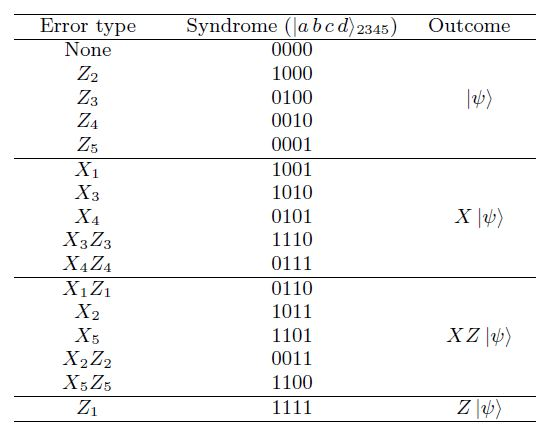
\includegraphics[scale=0.75]{gfx/error_table.JPG}
\caption{Error correction table based on outcomes in auxiliary qubits \citep{joo_error-correcting_2009}}
\label{fig:m_table}
\end{figure}

This process is also represented with a corresponding circuit model in Joo's paper \citep{joo_error-correcting_2009}, included here in figure \ref{fig:m_circuit} to facilitate understanding of the table.

\begin{figure}
\centering
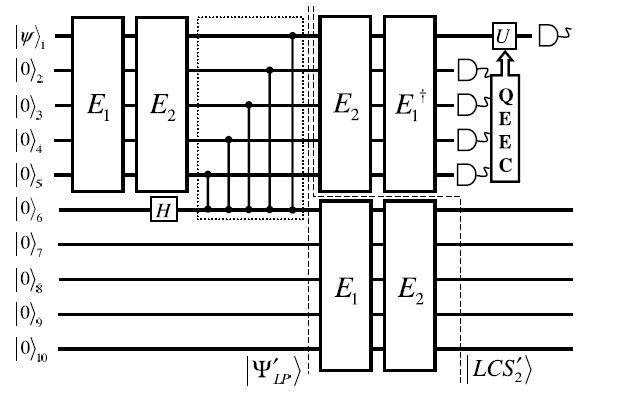
\includegraphics[scale=0.75]{gfx/error_circuit.JPG}
\caption{Full error correction circuit \citep{joo_error-correcting_2009}}
\label{fig:m_circuit}
\end{figure}

%----------------------------------------------------------------------------------------

\section{Higher Complexities}

One of the advantages of this error correction scheme is that it can be easily scaled for the encoding of higher numbers of qubits in each logical state. The conversion for this is simply to scale all operators that act on all three qubits to operate on the number of qubits in the new logical state. The effect of this should be a higher degree of fault tolerance when the error correction scheme is applied.

